\documentclass[aspectratio=169]{beamer}

% Pacotes essenciais
\usepackage[utf8]{inputenc}
\usepackage[T1]{fontenc}
\usepackage[brazilian]{babel}
\usepackage{graphicx}
\usepackage{tikz}

% Fonte moderna Roboto
\usepackage[sfdefault]{roboto}
\usepackage[T1]{fontenc}

% Definição das cores
\definecolor{vermelhoPrincipal}{HTML}{b11116}
\definecolor{azulComplementar}{HTML}{3a5461}
\definecolor{brancoFundo}{HTML}{FFFFFF}

% Configuração do tema
\usetheme{Madrid}
\usecolortheme{default}

% Cores personalizadas - texto sempre em preto
\setbeamercolor{structure}{fg=black}
\setbeamercolor{palette primary}{bg=vermelhoPrincipal,fg=white}
\setbeamercolor{palette secondary}{bg=azulComplementar,fg=white}
\setbeamercolor{palette tertiary}{bg=vermelhoPrincipal,fg=white}
\setbeamercolor{palette quaternary}{bg=azulComplementar,fg=white}
\setbeamercolor{frametitle}{bg=vermelhoPrincipal,fg=white}
\setbeamercolor{background canvas}{bg=brancoFundo}
\setbeamercolor{title}{fg=black}
\setbeamercolor{subtitle}{fg=azulComplementar}
\setbeamercolor{author}{fg=black}
\setbeamercolor{date}{fg=black}
\setbeamercolor{itemize item}{fg=black}
\setbeamercolor{itemize subitem}{fg=black}
\setbeamercolor{enumerate item}{fg=black}
\setbeamercolor{block title}{bg=vermelhoPrincipal,fg=white}
\setbeamercolor{block body}{bg=vermelhoPrincipal!10,fg=black}
\setbeamercolor{normal text}{fg=black}

% Configurar fonte dos itemize
\setbeamerfont{itemize/enumerate body}{size=\scriptsize}
\setbeamerfont{itemize/enumerate subbody}{size=\scriptsize}

% Marcadores modernos e minimalistas
\setbeamertemplate{itemize item}{\raisebox{0.2ex}{\rule{0.6ex}{0.6ex}}}
\setbeamertemplate{itemize subitem}{\raisebox{0.3ex}{\rule{0.4ex}{0.4ex}}}
\setbeamertemplate{itemize subsubitem}{\raisebox{0.35ex}{\rule{0.3ex}{0.3ex}}}
\setbeamertemplate{enumerate items}[square]

% Transições suaves
\setbeamercovered{transparent}

% Remover símbolos de navegação
\setbeamertemplate{navigation symbols}{}

% Customizar o cabeçalho com barra vermelha e logo
\setbeamertemplate{headline}{
  \begin{beamercolorbox}[wd=\paperwidth,ht=0.6cm,dp=0.15cm,leftskip=0.2cm,rightskip=0.4cm]{palette primary}
    \raisebox{-0.05cm}{
\includegraphics[height=0.45cm]{imgs/base/fatec-rgt.png}}
    \hfill
    \raisebox{-0.18cm}{
\includegraphics[height=0.85cm]{imgs/base/governo-sp-secretaria-logo.png}}
    \hspace{0.2cm}
    \raisebox{-0.08cm}{
\includegraphics[height=0.6cm]{imgs/base/cps-logo.png}}
  \end{beamercolorbox}
}
% Remover sombras dos blocks
\setbeamertemplate{blocks}[default]
\setbeamertemplate{itemize/enumerate body begin}{\scriptsize}
\setbeamertemplate{itemize/enumerate subbody begin}{\scriptsize}
% Customizar o rodapé
\setbeamertemplate{footline}{
  \begin{beamercolorbox}[wd=\paperwidth,ht=0.4cm,dp=0.2cm,leftskip=0.3cm,rightskip=0.3cm]{palette secondary}
    \usebeamerfont{footline}
    \insertshortauthor \hfill \hfill {\fontsize{5}{6}\selectfont\insertshorttitle} \hfill \hfill \insertframenumber/\inserttotalframenumber
  \end{beamercolorbox}
}

% Customizar título do frame
\setbeamertemplate{frametitle}{
  \vspace{0.3cm}
  \textcolor{black}{\insertframetitle}
  \vspace{0.1cm}
}

% Informações da apresentação
\title{Criação de Camarão em Cativeiro com \\Monitoramento IoT para Gastronomia}
\subtitle{}
\author[DSM]{ALMEIDA, D.; MUNIZ, L.; RODRIGUES, T.}
\institute{Desenvolvimento de Software Multiplataforma\\FATEC Registro}
\date{\today}

\begin{document}

% Slide de título moderno
\begin{frame}
  \vspace{0.8cm}
  \begin{center}
    \begin{tikzpicture}
      % Linha decorativa superior
      \draw[vermelhoPrincipal, line width=2pt] (-4,0) -- (4,0);
    \end{tikzpicture}
    
    \vspace{0.4cm}
    
    {\normalsize\bfseries\inserttitle}\par
    
    \vspace{0.2cm}
    
    {\tiny\insertauthor}\par
    
    \vspace{0.1cm}
    
    {\small\textcolor{azulComplementar}{\insertsubtitle}}\par
    
    \vspace{0.5cm}
    
    \begin{tikzpicture}
      % Linha decorativa inferior
      \draw[azulComplementar, line width=1.5pt] (-2.5,0) -- (2.5,0);
    \end{tikzpicture}
    
    \vspace{0.3cm}
    
    {\scriptsize\insertinstitute}\par
    
    \vspace{0.01cm}
    
    {\tiny\textcolor{azulComplementar}{\insertdate}}\par
  \end{center}
\end{frame}

\section{Agenda}
{
\usebackgroundtemplate{%
  
\includegraphics[width=\paperwidth,height=\paperheight]{imgs/teste.png}%
}

% Slide de agenda
\begin{frame}[b]{Agenda}
  \begin{itemize}
    \item Pitch
    \item Problematização
    \item Estado da Arte
    \item Objetivo
    \item Ferramental
    \item Metodologia
    \item Apresentação prática
    \item Resultados e Discussões
  \end{itemize}
  
  \vfill
  
  \hfill{\scriptsize \textbf{Duração:} 10 a 11 min.}
\end{frame}

\section{Pitch}
{
\usebackgroundtemplate{%
  
\includegraphics[width=\paperwidth,height=\paperheight]{imgs/LOGO.png}%
}
\begin{frame}[b]{Pitch}

\end{frame}
}

\section{Problematização}

{
\usebackgroundtemplate{%
  
\includegraphics[width=\paperwidth,height=\paperheight]{imgs/teste.png}%
}
\begin{frame}[b]{Problematização}
  \begin{itemize}
    \item \parbox{0.60\textwidth}{Manejo predominantemente manual}
    \item \parbox{0.60\textwidth}{Ausência de controle automatizado}
    \item \parbox{0.60\textwidth}{Falta de registro histórico dos parâmetros ambientais}
  \end{itemize}
  
  \vfill
  
  {\fontsize{4}{5}\selectfont\textit{Fonte: Seu Nome}\hfill\textcolor{white}{Imagem: Descrição da imagem}}
\end{frame}
}

\section{Estado da Arte}

{
\usebackgroundtemplate{}
\begin{frame}[t]{Estado da Arte}

\begin{table}
    \centering
    \tiny
    \begin{tabular}{|p{2.5cm}|p{2cm}|p{2cm}|p{2cm}|p{2cm}|p{1.5cm}|}
      \hline
      \textbf{Título/Autores} & \textbf{Objetivo} & \textbf{Método} & \textbf{Resultados} & \textbf{Limitações} & \textbf{Gap} \\
      \hline
      Sistema de telemonitoramento para carcinicultura — Dantas (2020) & Monitorar temperatura, pH e oxigênio dissolvido em viveiros de camarão & ESP32 com LoRaWAN e integração AWS via MQTT & Variação de 0,5°C na temperatura e alcance de 138 metros & Ausência de monitoramento de amônia e baixa autonomia energética & Sem controle de alimentação e sem registro histórico \\
      \hline
      Monitoramento em tempo real para fazendas de camarão de água doce — Uddin (2020) & Monitorar qualidade da água e taxa de sobrevivência em cultivo real & Arduino Yun com sensores múltiplos, método AHP em nuvem e notificações web & 4.600+ registros, erro inferior a 7\%, sobrevivência de 90\% & Dependência exclusiva de Wi-Fi e necessidade de calibração manual frequente & Sem automação da alimentação e sem monitoramento de amônia \\
      \hline
      Monitoramento via rede de sensores sem fio em viveiro de vannamei — Zainuddin (2019) & Monitorar temperatura, pH e turbidez em múltiplos pontos do viveiro & WSN com Atmega 2560/328, módulos Xbee (Zigbee) e ESP8266 & Acurácia de 97,75\% para temperatura, 98,85\% para pH e 99,73\% para turbidez & Sem redundância de hardware e limitações de escalabilidade & Sem controle de alimentação e sem alertas preventivos \\
      \hline
    \end{tabular}
  \end{table}
\end{frame}
}

\section{Objetivo}

{
\usebackgroundtemplate{%
  
\includegraphics[width=\paperwidth,height=\paperheight]{imgs/teste.png}%
}
\begin{frame}[b]{Objetivo}
  \begin{itemize}
    \item \parbox{0.60\textwidth}{\textbf{Objetivo geral}: Desenvolver um sistema de monitoramento automatizado para cativeiros de camarão.}
    \item \parbox{0.60\textwidth}{\textbf{Objetivos específicos}:}
    \begin{itemize}
      \item \parbox{0.55\textwidth}{Monitorar remotamente os parâmetros ambientais (temperatura, pH, amônia)}
      \item \parbox{0.55\textwidth}{Registrar e armazenar dados históricos dos cativeiros}
      \item \parbox{0.55\textwidth}{Automatizar o fornecimento de ração}
      \item \parbox{0.60\textwidth}{Disponibilizar uma aplicação web responsiva}
    \end{itemize}
  \end{itemize}
  
  \vfill
  
  {\fontsize{4}{5}\selectfont\textit{Fonte: Seu Nome}\hfill\textcolor{white}{Imagem: Descrição da imagem}}
\end{frame}
}

\section{Ferramental}

{
\usebackgroundtemplate{%
  
\includegraphics[width=\paperwidth,height=\paperheight]{imgs/teste.png}%
}
\begin{frame}[b]{Ferramental}
  \begin{itemize}
  \item \parbox{0.60\textwidth}{\textbf{Linguagens}: JavaScript, TypeScript, Arduino/C++}
  \item \parbox{0.60\textwidth}{\textbf{Frameworks}: Express.js, Next.js 14, React 18, Mongoose}
  \item \parbox{0.60\textwidth}{\textbf{Banco de dados}: MongoDB Atlas (cloud)}
  \item \parbox{0.60\textwidth}{\textbf{Infraestrutura}: Docker,Node.js 18+, Alpine Linux}
  \item \parbox{0.60\textwidth}{\textbf{Ferramentas}: Git, Vercel, Render Swagger/OpenAPI 3.0}
  \item \parbox{0.60\textwidth}{\textbf{APIs e integrações utilizadas}: Nodemailer, MongoDB Atlas API, NTP Server, Web Push API, JWT, Axios, DallasTemperature, OneWire, HTTPClient}
  \end{itemize}
  
  \vfill
  
  {\fontsize{4}{5}\selectfont\textit{Fonte: Seu Nome}\hfill\textcolor{white}{Imagem: Descrição da imagem}}
\end{frame}
}

\section{Metodologia}

{
\usebackgroundtemplate{}
\begin{frame}[t]{Metodologia}
  \centering
  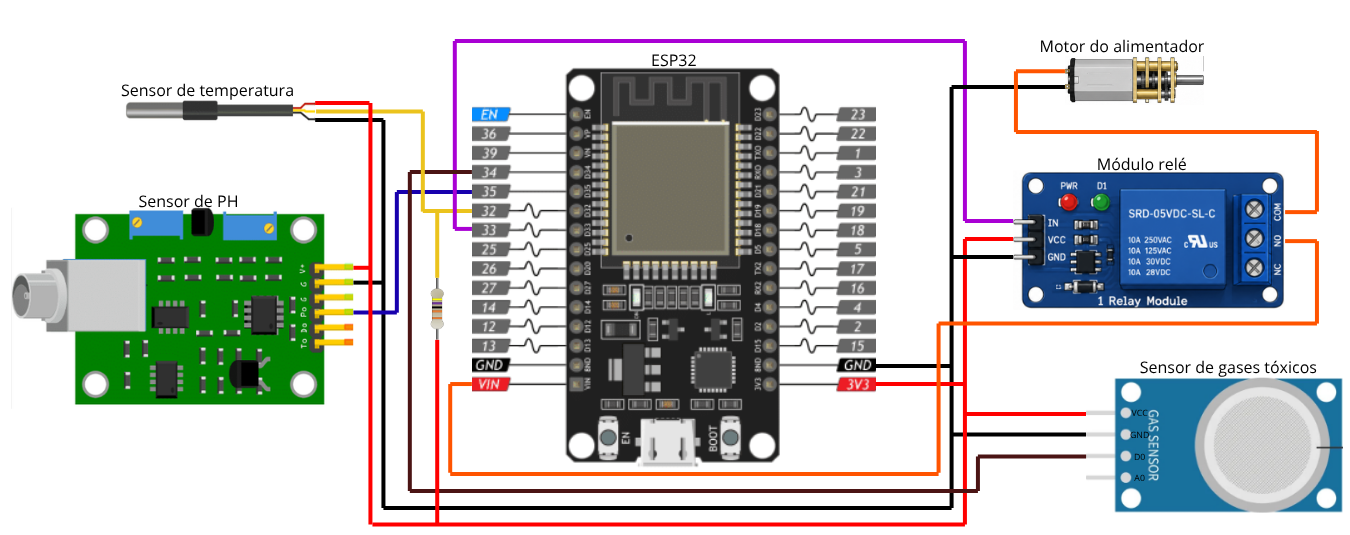
\includegraphics[width=0.8\paperwidth,keepaspectratio]{imgs/diagrama-iot-camarize.png}
\end{frame}
}

{
\usebackgroundtemplate{}
\begin{frame}[t]{Metodologia}
  \centering
  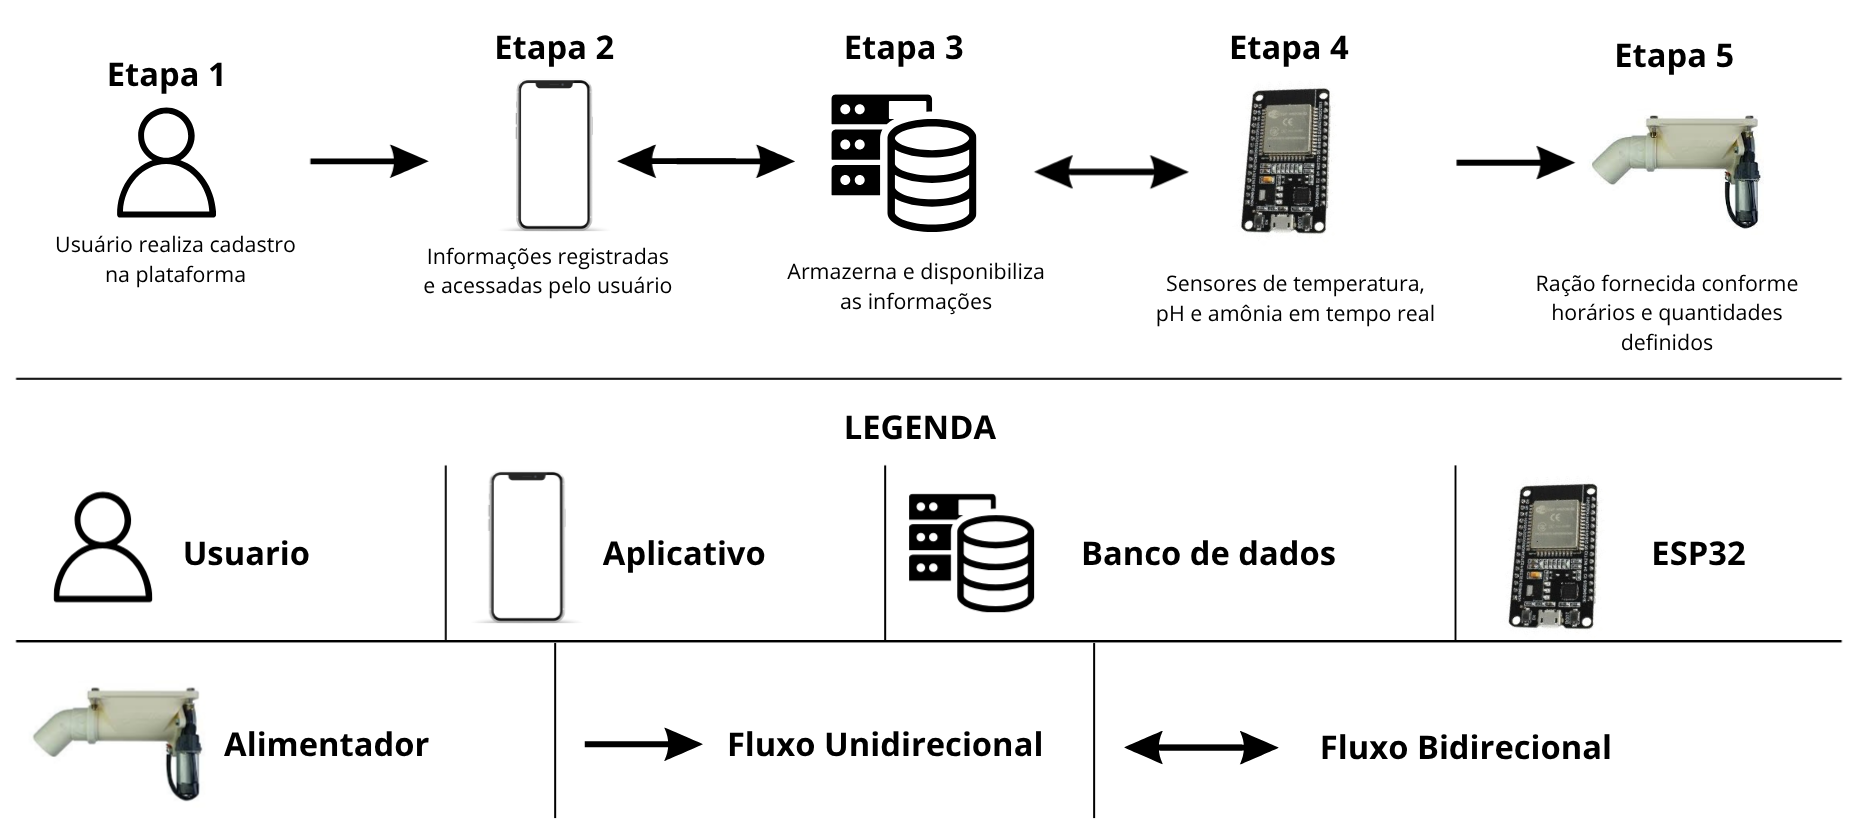
\includegraphics[width=0.8\paperwidth,keepaspectratio]{imgs/fluxograma-camarize.png}
\end{frame}
}

\section{Apresentação Prática}

{
\usebackgroundtemplate{%
  
\includegraphics[width=\paperwidth,height=\paperheight]{imgs/LOGO.png}%
}
\begin{frame}[b]{Apresentação Prática}
  
  \vfill
  
  {\fontsize{4}{5}\selectfont\textit{Fonte: Autoria Própria}\hfill\textcolor{white}{Imagem: Descrição da imagem}}
\end{frame}
}

\section{Resultados e Discussões}

{
\usebackgroundtemplate{}
\begin{frame}[t]{Resultados e Discussões}
  \begin{table}[H]
    \centering
    \resizebox{\textwidth}{!}{%
    \begin{tabular}{ccccccc}
      \hline
      \textbf{Teste} & \textbf{Temp. Real (°C)} & \textbf{Temp. Sensor (°C)} & \textbf{pH Real} & \textbf{pH Sensor} & \textbf{Amônia Real} & \textbf{Amônia Sensor} \\
      \hline
      1 & 21,0 & 20,50 & 7,0 & 6,79 & 0,000 & 0,000 \\
      2 & 26,0 & 25,79 & 7,0 & 6,79 & 0,000    & 0,000 \\
      3 & 17,0 & 16,80 & 7,0 & 6,79 & 0,000    & 0,000 \\
      4 & 21,0 & 20,50 & 5,0 & 4,80 & 0,000    & 0,000 \\
      5 & 22,0 & 21,60 & 8,6 & 7,90 & 0,000    & 0,000 \\
      6 & 22,0 & 21,60 & 7,0 & 6,79 & 0,000    & 0,000 \\
      \hline
      \textbf{Erro médio} & \multicolumn{2}{c}{\textbf{1,73\%}} & \multicolumn{2}{c}{\textbf{4,02\%}} & \multicolumn{2}{c}{—} \\
      \textbf{Precisão média} & \multicolumn{2}{c}{\textbf{98,27\%}} & \multicolumn{2}{c}{\textbf{95,98\%}} & \multicolumn{2}{c}{—} \\
      \hline
    \end{tabular}}
    \label{tab:sensores}
  \end{table}
\end{frame}
}

{
\usebackgroundtemplate{%
  
\includegraphics[width=\paperwidth,height=\paperheight]{imgs/teste.png}%
}
\begin{frame}[b]{Resultados e Discussões}
\begin{itemize}
  \item \parbox{0.60\textwidth}{Principais \textbf{resultados} alcançados: monitoramento em tempo real, alertas automáticos e controle remoto da alimentação}
  \item \parbox{0.60\textwidth}{Análise de \textbf{métricas}: precisão de 98,27\% (temperatura) e 95,98\% (pH), alertas em ~2 minutos}
  \item \parbox{0.60\textwidth}{Feedback dos \textbf{usuários}: 6 testes em ambiente real, interface aprovada em usabilidade}
  \item \parbox{0.60\textwidth}{\textbf{Desafios}: sensor MQ-135 limitado em meio aquático e instabilidade mecânica no dispensador}
  \item \parbox{0.60\textwidth}{Contribuições e \textbf{aprendizados}: viabilidade técnica de sistema IoT unificado de baixo custo}
  \item \parbox{0.60\textwidth}{\textbf{Trabalhos futuros}: sensor íon-seletivo submersível, redesenho do dispensador e validação em cativeiro comercial}
\end{itemize}
  
  \vfill
  
  {\fontsize{4}{5}\selectfont\textit{Fonte: Seu Nome}\hfill\textcolor{white}{Imagem: Descrição da imagem}}
\end{frame}
}

% Slide Informações Gerais (clone)
{
\usebackgroundtemplate{%
  
\includegraphics[width=\paperwidth,height=\paperheight]{imgs/obrigado.png}%
}
\begin{frame}[b]{}
  \vspace{0.2cm}
  
  \hspace*{0.25\paperwidth}
  
  \vfill
\end{frame}
}

\end{document}
